\documentclass[conference]{IEEEtran}

\usepackage{textcomp}
%\usepackage{algorithmic}
\usepackage{cite}
\usepackage{times}
\usepackage[ruled,noresetcount,noend]{algorithm2e}
\usepackage{graphicx}
\usepackage{url}\renewcommand{\baselinestretch}{1}
\usepackage{epsfig}
\usepackage{epstopdf}
\usepackage{amsmath,amssymb,amsfonts}
\usepackage{amsmath}
\usepackage{multirow}
%\usepackage{caption}
\usepackage{fancyvrb}
\usepackage{alltt}
\usepackage{caption}
\usepackage{mathptmx}
\usepackage{alltt}
\usepackage[switch, modulo]{lineno}
\usepackage{algpseudocode}
\usepackage{booktabs}
\usepackage{slashbox,pict2e}
\usepackage{array}
\usepackage[normalem]{ulem}
\usepackage{subcaption}
\usepackage{url}
\usepackage{kbordermatrix}% http://www.hss.caltech.edu/~kcb/TeX/kbordermatrix.sty
 \usepackage{graphicx}

\newtheorem{theorem}{Theorem}
\setcounter{theorem}{0}
%\theoremstyle{definition}
\newtheorem{definition}{Definition}
\setcounter{definition}{0}
%\theoremstyle{remark}
\newtheorem{remark}{Remark}
\newtheorem{lemma}[theorem]{Lemma}
%s\newtheorem*{cor}{Corollary}
%\theoremstyle{property}
\newtheorem{example}{Example}
\newtheorem{property}{Property}
\setcounter{property}{0}
\newtheorem{condition}{C}
\setcounter{condition}{0}
\newtheorem{conditions}{Condition}
\setcounter{conditions}{0}

\usepackage{caption}
\DeclareCaptionFont{ninept}{\fontsize{8pt}{11pt}\selectfont #1}
\captionsetup{font=ninept}




\begin{document}
%
% paper title
% can use linebreaks \\ within to get better formatting as desired
\title{A Trust-based Game Theoretical Model for Cooperative Intrusion Detection in Multi-cloud Environments}


% author names and affiliations
% use a multiple column layout for up to two different
% affiliations

\author{
\IEEEauthorblockN{Adel Abusitta, Martine Bellaiche, and Michel Dagenais}
\IEEEauthorblockA{\textit{Department of Computer and Software Engineering}\\
 \textit{Ecole Polytechnique de Montr´eal}\\
Montr´eal, Canada}

\{adel.abusitta,martine.bellaiche,michel.dagenais\}@polymtl.ca}

% make the title area
\maketitle


\begin{abstract}
Cloud systems are becoming more complex and vulnerable to attacks. Cyber attacks are also becoming more sophisticated and harder to detect. Therefore, it is increasingly difficult for a single cloud-based intrusion detection system (IDS) to detect all attacks, because of limited and incomplete knowledge about attacks. The recent researches in cyber-security have shown that a cooperation among IDSs can bring higher detection accuracy in such complex computer systems. Through collaboration, a cloud-based IDS can consult other IDSs about suspicious intrusions and increase the decision accuracy. The problem of existing cooperative IDS approaches is that they overlook having untrusted (malicious or not) IDSs that may negatively effect the decision about suspicious intrusions in the cloud. Moreover, they rely on a centralized architecture in which a central agent regulates the cooperation, which contradicts the distributed nature of the cloud. In this paper, we propose a framework that enables IDSs to distributively form trustworthy IDSs communities. We devise an algorithm, based on cooperative game theory, that allows a set of cloud-based IDSs to cooperatively set up their coalition in such a way to make their individual detection accuracy increase, even in the presence of untrusted IDSs.

\end{abstract}

\begin{IEEEkeywords}
Intrusion detection systems; game theory; cloud computing; security; trust.
\end{IEEEkeywords}


% For peer review papers, you can put extra information on the cover
% page as needed:
% \ifCLASSOPTIONpeerreview
% \begin{center} \bfseries EDICS Category: 3-BBND \end{center}
% \fi
%
% For peerreview papers, this IEEEtran command inserts a page break and
% creates the second title. It will be ignored for other modes.
\IEEEpeerreviewmaketitle



\section{Introduction}

Cloud-based cyber-attacks are known to be more complex and harder to detect. It became significantly more difficult for a traditional single intrusion detection system, whether it is network-based, hypervisor-based, or VM-based, to detect all attacks, due to limited knowledge about attacks. Collaboration among intrusion detection systems (IDSs) can be used to gain higher detection accuracy as compared to traditional single IDS. Through collaboration, IDSs in different regions, and possibly, belonging to different Cloud Providers (CPs) can cooperate in such a way that makes them utilize the expertise of each other to cover and identify unknown attack patterns.

A cloud-based IDS can be classified into two types; signature-based and anomaly-based \cite{modi2013survey}. The former compares suspicious behavior with known attack patterns. In order to make signature-based effective, the signature database should be updated frequently.  On the other hand, anomaly-based IDS raises alarms when unusual and/or unexpected observations are detected. Anomaly-based IDSs are effective to detect unknown attacks. Moreover, they do not need a database of known attacks. However, the shortcoming of using anomaly-based detection is the relative high false positive rate compared to the signature-based technique \cite{fung2016facid}. IDSs may adopt both techniques to have improved detection accuracy. However, the detection accuracy is limited by the amount of knowledge they have (e.g., their security vendors have). Recent research \cite{fung2016facid} \cite{fung2014revmatch} shows that the collaborative detection can enhance the detection rate up to 60\%. Through collaboration, an IDS can benefit from other IDSs expertise by consulting them about suspicious behavior. The feedback received can be then used to decide whether to rise an alarm or not. %\\

The main limitation of existing cloud-based cooperative IDS (e.g.  \cite{man2012collaborative} \cite{singh2016collaborative} \cite{ghribi2016distributed} \cite{chiba2016cooperative} \cite{al2015cl} \cite{kholidy2012cids}) is that they work under the assumption that all IDSs are trustable, which lets their collaboration systems vulnerable to untrusted (malicious or not) insiders.%\\

To address the aforementioned problems, we propose a trust-based framework for cooperative IDS in a multi-cloud environment. The framework can be summarized as follows. We enable an IDS to evaluate other IDSs' trustworthiness. This is done by considering its personal experience using bayesian inference. After obtaining IDSs' trust values, a coalition formation algorithm is used, that is based on the coalitional game theory \cite{ray2007game}. The algorithm enables IDSs to leave or join a given coalition in such a way that enhances its chance to work with trusted IDSs. Thereafter, we propose a feedback aggregation algorithm, that is based on the Dempster-Shafer Theory (DST) \cite{shafer1992dempster}, to enable an IDS inside a coalition to aggregate feedbacks from different IDSs about suspicious intruders, which helps make the optimal decision in terms of detection accuracy.

Unlike similar proposals (e.g. \cite{dermott2015collaborative}), we adopt a distributed
approach in which each IDS autonomously makes its own decisions. This, in turn, avoids the difficulty of finding a third party that is trusted by all the IDSs. Also, it reduces the instability inside the coalition due to a single point of failure. In summary, our work consists of the following contributions:

\begin{itemize}

\item  Modeling and proposing a framework that enables cloud-based IDSs to distributively form trustworthy IDS communities. More specifically, we present a systematic approach that considers the trustworthiness of IDSs through creating cooperative IDS.

\item Proposing a new trust evaluation approach, based on Bayesian inference, that enables a cloud-based IDS to evaluate another IDS's trustworthiness based on its personal experiences.

\item Devising an algorithm, based on cooperative game theory, that allows a set of cloud-based IDSs to cooperatively set up their coalition in such a way to increase their individual detection accuracy in the presence of untrusted IDSs. The proposed algorithm converges to a Nash-stable situation; that is, no IDS has an incentive to leave its current coalition to move to another coalition.
\end{itemize}

The rest of this paper is organized as follows. In Section II, we discuss the related work. We present the trust-based cooperative intrusion detection system in Section III. In Section IV, we present our empirical results to show the effectiveness of the proposed approach. Finally, Section V concludes the paper.


\section{Related Work}

Cloud-based cooperative IDSs have been proposed in many works in the past. For example, Lo et al. \cite{lo2010cooperative} propose a cooperative detection approach within the cloud computing environment. Alerts are exchanged between the cloud environment nodes (i.e., hosts) whenever an attack gets detected. They use a rule-based technique to detect TCP SYN attacks by fetching the threshold for rule patterns through the initial rule establishment phase. The main advantage of this approach is that it is able to distribute the detection overhead between the cloud nodes. Recently, Teng et al. \cite{teng2014cooperative} proposed an approach that combines two detectors: a feature detector and a statistical detector. The feature detector uses SNORT to separate events based on network protocols (e.g., TCP). The statistical detector cooperates with the feature detector by using data packets from it to determine whether an event is an attack or not. If the rate of packets obtained exceeds the predefine threshold, then this case will be considered as an attack.

Man and Huh \cite{man2012collaborative} and Singh et al. \cite{singh2016collaborative} proposed a cooperative IDS between cloud computing regions. Their method allows exchanging alerts from multiple elementary detectors. In addition, they enable the exchange of knowledge between interconnected clouds. Ghribi \cite{ghribi2016distributed}  proposed a  middleware IDS. The approach enables a cooperation between cloud IDS layers: Hybervisor-based IDS, Network-based IDS and VM-based IDS. If an attack is detected in a layer, the attack cannot be executed in the other layers. Chiba et al. \cite{chiba2016cooperative}  introduced a cooperative network-based cooperative intrusion detection system to identify network attacks in the cloud environment. This can be done by monitoring network traffic while maintaining performance and service quality.

The main limitation of the above mentioned approaches is that they work in the assumption that all IDSs are trustable, which makes their collaboration systems vulnerable to malicious insiders. The aim of this paper is to present a systematic approach to build a cloud-based cooperative IDS that adopts trust assessment mechanisms and supports trustworthy aggregation decisions. The proposed approach should work in the presence of untrusted cloud-based IDSs .

In a multi-cloud environment, Dermott et al. \cite{dermott2015collaborative} proposed a cooperative intrusion detection in federated cloud environments. They use the Dempster-Shafer theory of evidence to collect the beliefs provided by the watching entities. The collected beliefs are used to make the final decision regarding a possible attack. The main limitation of this approach is that it is based on a centralized architecture, whereby a trusted third-party called broker is responsible for collecting feedback and managing intrusion detection.

In a non-cloud environment, a cooperative IDS has also been recently proposed in \cite{locasto2005towards} \cite{cordero2015community} \cite{yegneswaran2004global} \cite{cai2005collaborative} \cite{liu2015collaborative} \cite{patel2017nifty} \cite{huang2015openflow} \cite{sedjelmaci2015accurate}. However, these works also have the limitation of the above mentioned approaches, since they rely on the assumption that all IDSs are trustable, which makes their collaboration system vulnerable to malicious insiders.

A trust-based cooperative IDS has been proposed in a non-cloud environment. For example, Fung and Zhu \cite{fung2016facid} present a trust-based collaborative decision framework. Through cooperation, a local  intrusion detection system (IDS) can detect new attacks that may be known to other IDSs, which may be from different security vendors. They study how to utilize the diagnosis from different IDSs to perform intrusion detection. They present a system architecture of a collaborative IDS in which trustworthy feedback aggregation is a key component. Similarly, Zhu et al. \cite{zhu2009game} \cite{zhu2012guidex} proposed an incentive-based communication protocol, which provides IDS nodes incentives to send feedbacks to their peers, and thus to prevent malicious behaviors. The main limitation of the existing trust-based cooperative IDS is that it considers a consultation request to be sent to many IDSs in order to get a feedback. This in turn causes extra overhead, through consulting needlessly some IDSs (i.e., untrusted IDSs). This is unlike our approach, where we use a coalitional game, in order to construct a set of trusted IDSs and thus minimise the number of consultation requests while guaranteeing higher detection accuracy.

In general, for a multi-cloud environment, a decentralized framework that considers trustworthiness of IDSs during the cooperation had yet to be addressed. Thus, in this paper, we present a trust-based cooperative IDS in a multi cloud environment. This in turn, enhances the detection accuracy compared to the existing cooperative and non-cooperative IDSs.

\section{The Proposed Trust-based Cooperative IDS}

In this section, we present a trust-based cooperative IDS in a multi-cloud environment. The section is divided into the following subsections: trust evaluation, trust-based coalition formation algorithm and feedback aggregation (Fig. \ref{fig1}).


\begin{figure}[!ht]

\centering
\scalebox{0.55}{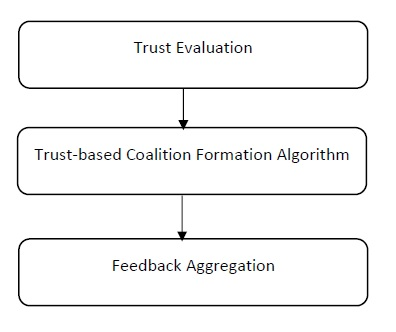
\includegraphics{frm.jpg}}
\caption{Proposed Methodology}
\label{fig1}
\end{figure}

\subsection{Trust Evaluation}

A cloud-based IDS can evaluate the trust value of another IDS based on its personal experience with that IDS. We adopt
a Bayesian inference approach to compute the trust value of an IDS \cite{josang2002beta}. The Bayesian inference was chosen because it is well-founded to derive trust values \cite{yahyaoui2012trust}. When the cloud-based IDS consults another IDS regarding a suspicious intruder, the received feedback and the revealed result (i.e., attack or not) are used to update the trust value of the consulted IDS. The trust value can be promoted if the IDS successfully diagnosed the consultation request about a suspicious intruder and it can be demoted otherwise. The trust value here represents and shows the accuracy of the IDS diagnosing suspicious attacks. An IDS $i$ $\in$ $\mathcal{N}$, where $\mathcal{N}$  is a set of IDSs, is endowed with a belief function, which computes the trust level of another IDS $j$ $\in$ $\mathcal{N}$. The
new trust value $t'_{j}$ is derived from the old trust value $t_{j}$ as follows:

\begin{equation}
t'_{j}=F(t_{j};\alpha_{j},\beta_{j})
\end{equation}

where $F$ is the regularized incomplete beta function
\cite{josang2002beta}, which is also the cumulative beta distribution function
of the following beta probability density function:
\begin{equation}
f(x;\alpha_{j},\beta_{j})=\frac{x^{\alpha_{j}-1}(1-x)^{\beta_{j}-1}}{\mathbf{B}(\alpha_{j},\beta_{j})}
\end{equation}

$\mathbf{B}$ represents the complete beta function. The value of $\alpha_{j}$ and
$\beta_{j}$ are updated after receiving the feedback from
an IDS $j$. $\beta_{j}$ is increased when the IDS $j$
successfully diagnoses the consultation request. Equation (4) describes the
update of $\beta_{j}$.

\begin{equation}
\beta_{j} = \beta_{j} \times (1+\rho_{j})
\end{equation}

where $\rho_{j}$ represents the weight of the diagnosed consultation request
if it is successful and 0 if not.

Equation (4) describes the update of $\alpha_{j}$.

\begin{equation}
\alpha_{j} = \alpha_{j} \times (1+\gamma_{j})
\end{equation}

where $\gamma_{j}$ denotes the weight of the diagnosed consultation request
if it is unsuccessful and 0 if not.

The values of $\rho_{j}$ and $\gamma_{j}$ should be carefully set by an IDS $i$ who is requesting feedback about a suspicious attack from other IDSs. These values reflect the detection difficulty degree of the suspicious intruder. The higher value of $\beta_{j}$ will increase the trust of an IDS $j$ while a higher value of $\alpha_{j}$ will decrease it.

The initial trust value $t_{j}$ is obtained at the beginning during the testing period. The total reported diagnosis data from peer IDS $j$ is denoted by the set $\mathcal{M}_{j}$. The initial trust value represents the total number of consultation requests that have been successfully diagnosed over the total number of consultation requests:

\begin{equation}
t_{j}=\frac{\sum_{k \in \mathcal{M}_{j}} r_{j,k}}{|\mathcal{M}_{j}|}
\end{equation}

Where the parameter $r_{j,k}$ is the revealed result of the k-th diagnosis request: $r_{j,k}$ =1 indicates successful diagnosis of the k-th request. $r_{j,k}$ =0 indicates otherwise.

The initial value of $\alpha$ and $\beta$ can be obtained as follows:

\begin{equation}
\alpha_{j}=\sum_{k \in \mathcal{M}_{j}} (1 - r_{j,k})
\end{equation}

\begin{equation}
\beta_{j}=\sum_{k \in \mathcal{M}_{j}} (r_{j,k})
\end{equation}

\subsection{A Trust-based Coalition Formation}

In this section, we model the problem of coperative
IDS as a coalition formation cooperative game with
non-transferable utility \cite{bogomolnaia2002stability}.

\subsubsection{Characterization}

The proposed coalition formation algorithm is a hedonic coalitional game \cite{bogomolnaia2002stability}, \cite{dreze1980hedonic} \cite{wahab2016towards} \cite{wahab2017optimal}, a category of coalition formation
games \cite{ray2007game}, \cite{dreze1980hedonic}, \cite{apt2009generic} in which each agent (i.e. IDS)
acts selfishly, and its preferences for
a coalition depend only on the members of that coalition. A hedonic game is used due to the fact that finding the optimal coalition structure, in coalition formation, is NP-complete \cite{sandholm1999coalition}. Therefore, a hedonic game, which satisfies stability
features was used. Stability indicates that none of the coalition members (i.e. IDSs) finds an incentive to leave its current coalition and join another one.

To establish the model, we need to define a preference relation so that each
IDS can order and compare all the possible coalitions it
belongs to and build preferences over them. For any IDS $i$ $\in$ $\mathcal{N}$, where $\mathcal{N}$ is a set of
IDSs, a preference relation $\succ_{i}$ is defined as a transitive
binary relation over the set of all coalitions that IDS $i$ can
form \cite{bogomolnaia2002stability}. Specifically, for any IDS $i$ $\in$ $\mathcal{N}$, and given two coalitions $C_{1}$, $C_{2}$, the notation $C_{1}$ $\succ_{i}$ $C_{2}$ means that IDS $i$ prefers being a member of $C_{1}$ rather than $C_{2}$. \\

In our coalition formation game, the preference
function of the IDSs can be defined as follows:

\begin{equation}
C_{1} \succeq_{i} C_{2} \Longleftrightarrow f_{i}(C_{1}) \geq f_{i}(C_{2})
\end{equation} \\

where $C_{1}$, $C_{2}$ $\subseteq$ $\mathcal{N}$ are two coalitions containing IDS $i$, and
$f_{i}(.)$ is a preference function defined as follows:

\begin{equation}
f_{i}(C_{k}) = U_{i}(C_{k}) = \prod _{j\in C_{k}} T_{i}^{j}
\end{equation}

$\prod _{j\in C _{k}} T_{i}^{j}$ is denoted as the coalition trust criterion. $T_{i}^{j}$ is denoted as IDS $i$ beliefs in IDS $j$ $\in$ $\mathcal{N}$.IDS $i$'s beliefs in $C_{k}$'s members is obtained using Bayesian inference as in (1). We use
the product of IDSs trust values instead of their summation in the definition of the coalition trust criterion in order to conserve the effect of small trust values on the global coalitions trust value. That way, the impact of a small trust value will not be mitigated by a higher one.


\subsubsection{The Proposed Coalition Formation Algorithm}

 The algorithm (Algorithm 1) that we propose is based on the hedonic shift rule \cite{bogomolnaia2002stability}: let
$\Pi = \{C_{1}, . . . , C_{l}\}$ represent the set of coalition partitions. That is, for k = $\{$1, 2, . . . , l$\}$, each $C_{k}$ $\subseteq$ $\mathcal{N}$ is a disjoint coalition. Each IDS $i$ $\in$ $\mathcal{N}$ decides to leave its current
coalition $C_{\Pi}(i)$ to join another one $C_{k} \in \Pi \cup \phi$ if and
only if its coalition trust criterion (i.e., $U_{i}(C_{k}) = \prod _{j\in C_{k}} T_{i}^{j}$) in
the new coalition exceeds the one it obtains in its
current coalition. Leaving and joining decisions are considered selfish decisions. This  means that they are made without considering their effect on the other IDSs.


%Algorithm here


\begin{algorithm}[h]
\SetKwInput{Initialization}{Initialisation}
\LinesNumbered
% \Initialization{}
\SetKwInOut{Input}{Input}\SetKwInOut{Output}{Output}
Given the current coalition partition $\Pi_{c} = \{C_{1}, . .
. , C_{l}\}$, each IDS $i$ evaluates possible shift from its
current coalition  as follows:

\Repeat{$\varepsilon$ elapses}
{
\ForEach{$C_{k} \in \Pi_{c} \cup \phi$}
{
\ForEach{IDS $j$ $\in C_{k}$}
{

\begin{itemize}
\item calculate the trust
value \\ of IDS $j$.
\end{itemize}

}
}
calculate $U_{i}(C_{k} \cup \{i\})$ and $U_{i}(C_{\Pi_{c}}(i))$

\uIf{$U_{i}(C_{k} \cup \{i\})$ $>$ $U_{i}(C_{\Pi_{c}}(i))$}
{


\begin{itemize}
\item IDS $i$ leaves its current \\ coalition $C_{\Pi_{c}}(i)$ and \\ joins the new coalition.

\item $\Pi_{c}$ is updated:

$\Pi_{c+1}$ =$(\Pi_{c}\setminus \{C_{\Pi_{c}}(i), C_{k}\})$ \\ $\cup \{C_{\Pi_{c}}({i}) \setminus \{{i}\}, C_{k} \cup \{{i}\}\}$.
\end{itemize}

\Else{
\begin{itemize}
\item IDS $i$ remains in the \\ same coalition so that:

$\Pi_{c+1} = \Pi_{c}$
\end{itemize}
}

}
}
\caption{Trust-based Coalition Formation Algorithm}
\end{algorithm}


In Algorithm 1, an IDS $i$ evaluates all of the possible coalitions
it can join or form, beginning by leaving its current coalition $C_{\Pi}$(i) to
join another already existing coalition $C_{k}$. The algorithm
computes the trust value for each IDS $j \in C_{k}$ as in (1). Then, the algorithm determines the coalition trust criterion $U_{i}(C_{\Pi}(i))$ of its current coalition $C_{\Pi}$(i) as in (9) and compares it with the coalition trust criterion $U_{i}(C_{k})$ of the coalition $C_{k}$. If the coalition trust criterion of the current coalition is greater than that of the coalition $C_{k}$, then the IDS $i$ leaves its current coalition to join $C_{k}$. Otherwise, IDS $i$ remains in its current coalition. One should note that, after a certain fixed period of time $\varepsilon$, the whole process is repeated, in order to obtain the changes that may happen in the current coalition partition $\Pi_{c}$. These changes include changes in the IDSs trust values, the departure of existing IDSs and the arrival of new IDSs.

The main complexity of Algorithm 1 lies in the shifting operations, i.e. the process of finding a new coalition to join,
which equals $O(|\Pi_{c}|)$, where $|\Pi_{c}|$ is the number of coalitions in the current coalition partition.

The algorithm can be implemented in a distributed
manner, given that each IDS can act autonomously and independently from any other IDSs in the system.
However, it is important to provide appropriate actions
based on \cite{guazzone2014game} for:

\begin{itemize}
\item State recovery: the algorithm assumes that each IDS
is able to retrieve the current coalition partition $\Pi_{c}$. Any
state retrieval algorithm available in the state-of-the-art (e.g. \cite{sinha1998distributed}, \cite{wooldridge2009introduction})
can be used for this purpose;
\item Atomic state update: to guarantee correctness, $\Pi_{c}$
must not change while IDS $i$ moves from its current coalition $C_{\Pi}$(i) and joins
another one. Distributed mutual exclusion algorithms (e.g. \cite{kshemkalyani2011distributed})
can be used for this purpose.

\end{itemize}
\subsection{Feedback Aggregation}

In the previous section, we presented a trust-based coalition formation model that enables a set of cloud-based IDSs to cooperatively set up their coalitions. The output of the coalition formation algorithm (Algorithm 1) is a set of coalitions, where each coalition consists of a set of IDSs that prefer to work with each other. In this section, we show how an IDS inside a coalition can aggregate feedbacks received from other IDSs in the same coalition. For this purpose, we use the Dempster-Shafer Theory (DST) for feedback aggregation. DST was selected for the following main reasons: (1) unlike other aggregation models (e.g. Bayesian aggregation model) that demand complete information of prior probabilities, DST can handle a lack of complete information (i.e. uncertainty), and (2) it has a property
to prevent collusion attacks, which occur when several malicious IDSs collaborate to give misleading judgments.

In our model, the frame of discernment, which describes the status of a suspicious intruder is $\Omega$= $\{1, 0 ,U\}$ denotes a set consisting of three hypotheses. $1$ means that IDS $j$ decides and
reports to IDS $i$ that there is an intrusion, $0$ means that IDS $j$ decides and
reports to IDS $i$ that there is no intrusion, and
$U$ shows that IDS $j$ is uncertain whether there is an intrusion or not.

DST combines multiple IDSs beliefs under the condition that evidences from different IDSs are independent. For example, if IDS $i$ wants to combine the belief of two IDSs $IDS_{1}$ and $IDS_{2}$ over the same frame of discernment  $\Omega$, the combined belief of $IDS_{1}$ and $IDS_{2}$ is calculated
as follows \cite{yu2002evidential}:

\begin{equation}
\begin{aligned}
&m_{IDS_{1}}(1)\oplus m_{IDS_{2}}(1) = \frac{1}{K}[m_{IDS_{1}}(1)m_{IDS_{2}}(1)+\\
&m_{IDS_{1}}(1)m_{IDS_{2}}(U)+m_{IDS_{1}}(U)m_{IDS_{2}}(1)] \\
\end{aligned}
\end{equation}

\begin{equation}
\begin{aligned}
&m_{IDS_{1}}(0)\oplus m_{IDS_{2}}(0) = \\
&\frac{1}{K}[m_{IDS_{1}}(0)m_{IDS_{2}}(0)\\
&+m_{IDS_{1}}(0)m_{IDS_{2}}(U)+m_{IDS_{1}}(U)m_{IDS_{2}}(0)] \\
\end{aligned}
\end{equation}

\begin{equation}
\begin{aligned}
m_{IDS_{1}}(U)\oplus m_{IDS_{2}}(U) =
\frac{1}{K}[m_{IDS_{1}}(U)m_{IDS_{2}}(U)]
\end{aligned}
\end{equation}

where,

\begin{equation}
\begin{aligned}
&K = m_{IDS_{1}}(1)+m_{IDS_{2}}(1)+m_{IDS_{1}}(1)+m_{IDS_{2}}(U)\\
&+m_{IDS_{1}}(U)+m_{IDS_{2}}(U)+m_{IDS_{1}}(U)+m_{IDS_{2}}(1)\\
&+m_{IDS_{1}}(U)+m_{IDS_{2}}(0)+m_{IDS_{1}}(0)+m_{IDS_{2}}(0)\\
&+m_{IDS_{1}}(0)+m_{IDS_{2}}(U)
\end{aligned}
\end{equation}

Here is an example. Assume the following:\\
$m_{IDS_{1}}(1)$ = 0.75 $m_{IDS_{1}}(0)$ = 0 $m_{IDS_{1}}(U)$ = 0.25\\
$m_{IDS_{2}}(1)$ = 0.6 $m_{IDS_{2}}(0)$ = 0 $m_{IDS_{2}}(U)$ = 0.4\\

by combining the above two belief functions, we can
obtain the result as follows: \\
$belief(1)=(0.75 \ast 0.6) + (0.75 \ast 0.4) + (0.6 \ast 0.25) = 0.9$\\
$belief(0) =(0 \ast 0) + (0 \ast 0.4) + (0 \ast 0.25) = 0$\\
$belief(U) =(0.25 \ast 0.4) = 0.1$\\
Since $belief(1)$ $>$ $belief(0)$ $>$ $belief(U)$, IDS $i$ will decide that an attack exists.


\section{Experimental Evaluation}
\label{sec:Experiments}
In this section, we first explain the experimental setup
used to perform our experimentation and then study the
performance of the proposed cooperative intrusion detection approach.

\subsection{Experimental Setup}

We implemented our framework in a 64-bit Windows 8 environment on a host equipped with an Intel Core i7-4790 CPU 3.60 GHz Processor and 16 GB RAM. We used Matlab for implementing our model.

The simulation environment uses 100 cloud-based IDSs. Each IDS is represented by two parameters, trust value $t$ and decision threshold $\tau$. The trust value represents the expertise level of the IDS, which in turn represents the ability of the IDS to catch suspicious traces from a given observation. The threshold $\tau$ represents the sensitivity of the IDS. Lower values of $\tau$ indicate a more sensitive IDS.

We use a Beta density function to reflect the intrusion detection capability of each IDS. A Beta density function is given by:

\begin{equation}
\begin{aligned}
f(z|\alpha,\beta)= \frac{1}{B(\alpha,\beta)z^{\alpha-1} (1-z)^{\beta-1}}\\
B(\alpha,\beta) = \int_{0}^{1} x^{\alpha-1}(1-x)^{\beta-1}dx
\end{aligned}
\end{equation}

\begin{equation}
\begin{aligned}
\alpha = 1 + \frac{t(1-d)}{d(1-t)}r \\
\beta = 1 + \frac{t(1-d)}{d(1-t)}(1-r)
\end{aligned}
\end{equation}

where $z$ $\in$ [0, 1] is the assessment result from the IDS about the likelihood of intrusion, and $f$ ($z$$|$$\alpha$,$\beta$) is the distribution of assessment $z$ from an IDS with trust level $t$ to an intrusion with difficulty level $d$ $\in$ [0, 1]. The trust level in the distribution can represent the expertise level of the IDS. Higher values of $d$ represent these attacks that are difficult to detect. Higher values of $t$ indicate a higher probability of generating correct intrusion assessments. $r$ $\in$ $\{$0, 1$\}$ is the expected result of detection. $r$ = 1 means that there is an intrusion and $r$ = 0 means otherwise.

In order to evaluate the ability of the proposed model in the presence of an untrusted environment, We made the percentage of untrusted IDSs 70\% (trust level $t$ $\leq$ 0.2). We argue, based on the recent literature \cite{wahab2015survey}, that the percentage of untrusted nodes tends to form the majority compared to that of trusted nodes. We applied the proposed coalition formation algorithm (Algorithm 1) on the considered IDSs.  We compared the proposed aggregation approach with other known aggregation approaches in the state-of-the-art: Majority aggregation model \cite{lo2010cooperative} and the weighted average aggregation model \cite{fung2009robust}. In the majority model, the IDS collects feedback from IDSs about suspicious behaviour and the decision is made (i.e., attack or not) according to the majority. However, in the weighted average aggregation model, weights $W$ are assigned to feedbacks from different IDSs to distinguish their detection capability. Highly trusted IDSs are assigned with larger weights compared to low trusted IDSs. The decision is made according to the following equation. If ($\Sigma_{k=1}^{n}$ $W_{k}y_{k}$) / ($\Sigma_{k=1}^{n}$ $W_{k}$) $\geq$ $\tau$, the decision is $\emph{the existence of an attack}$. Otherwise, the decision is that $\emph{there is no attack}$, where $W_{k}$ is the weight of the k-th IDS and $y_{k}$ is the feedback from the k-th IDS.


\subsection{Experimental Results}

In Fig. \ref{fig2}, we observe that the proposed aggregation model (i.e., Dempster-Shafer aggregation approach) shows significant improvement for the false negative rate, compared to the weighted and majority aggregation model at different threshold values $\tau$. Similarly, in Fig. \ref{fig3}, our model yields significant improvement for the false positive rate, compared to the other two models. This is justified by the fact that Dempster-Shafer disregards the untrustworthy feedbacks upon building the final decisions. Moreover, Dempster-Shafer gives a weight for each feedback according to the trustworthiness level of the IDS giving this feedback.

\begin{figure}[htbp]

\centering
\scalebox{0.45}{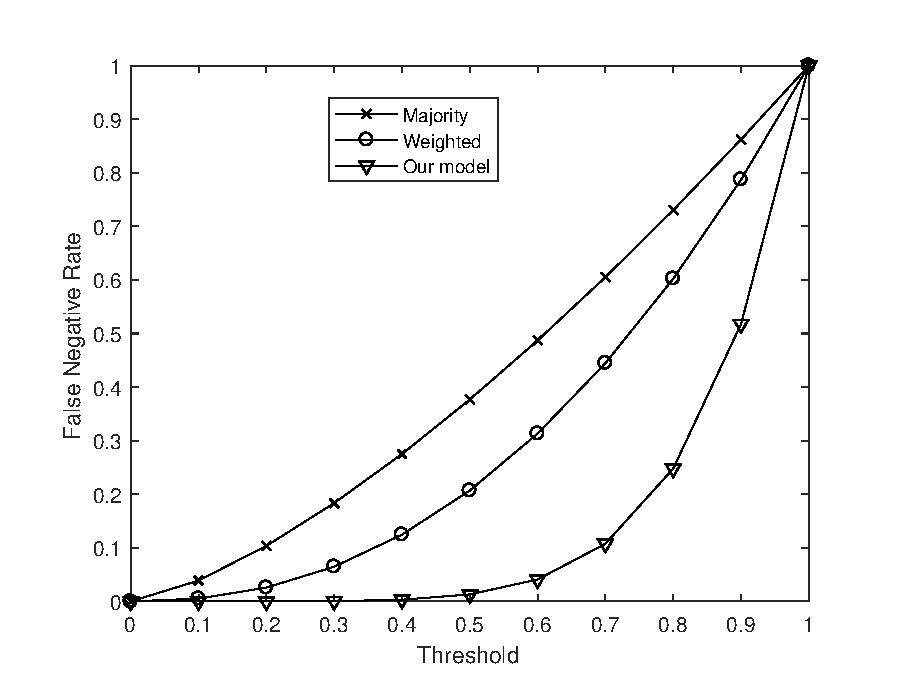
\includegraphics{fn.eps}}
\caption{Comparison of three aggregation models (False Negative Rate).}
\label{fig2}
\end{figure}

\begin{figure}[htbp]

\centering
\scalebox{0.45}{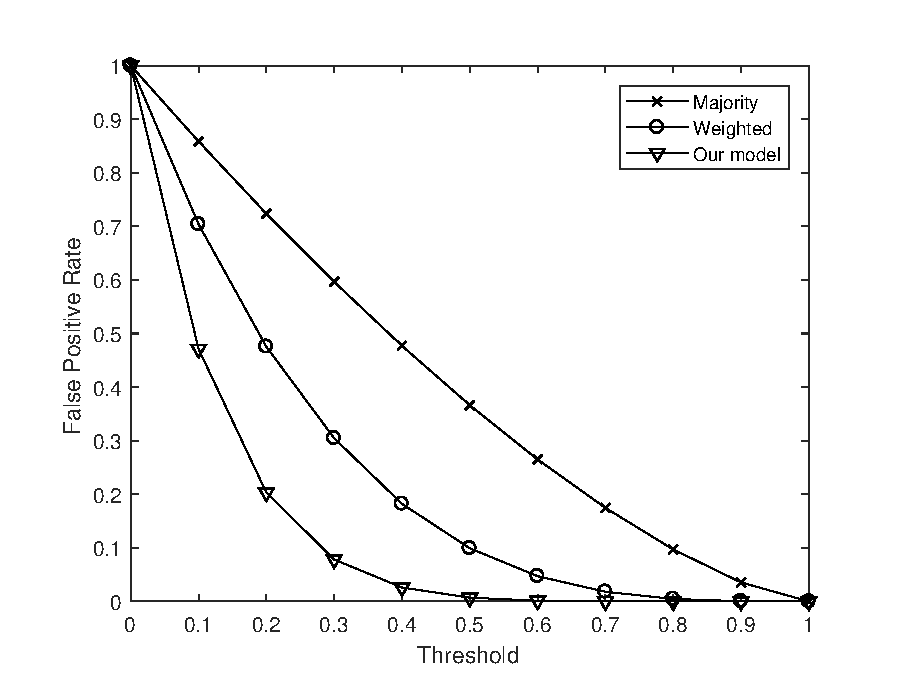
\includegraphics{fp.eps}}
\caption{Comparison of three aggregation models (False Positive Rate).}
\label{fig3}
\end{figure}


In Fig. \ref{fig4} and Fig. \ref{fig5}, we also study the effect of the trust value (i.e., expertise level) on the accuracy of the detection. To this end, we run our Algorithm (Algorithm 1) many times. Each time, we let IDSs have different values of $t$. The study is conducted at different threshold values $\tau$. Fig. \ref{fig4} shows that the false negative decreases when the trustworthiness level of an IDS increases. Similarly, Fig. \ref{fig5} shows that the false positive decreases when the trustworthiness level of an IDS increases. This is justified by the fact that whenever an IDS becomes more trusted, it will be able to give a right feedback about suspicious attacks.

\begin{figure}[htbp]

\centering
\scalebox{0.45}{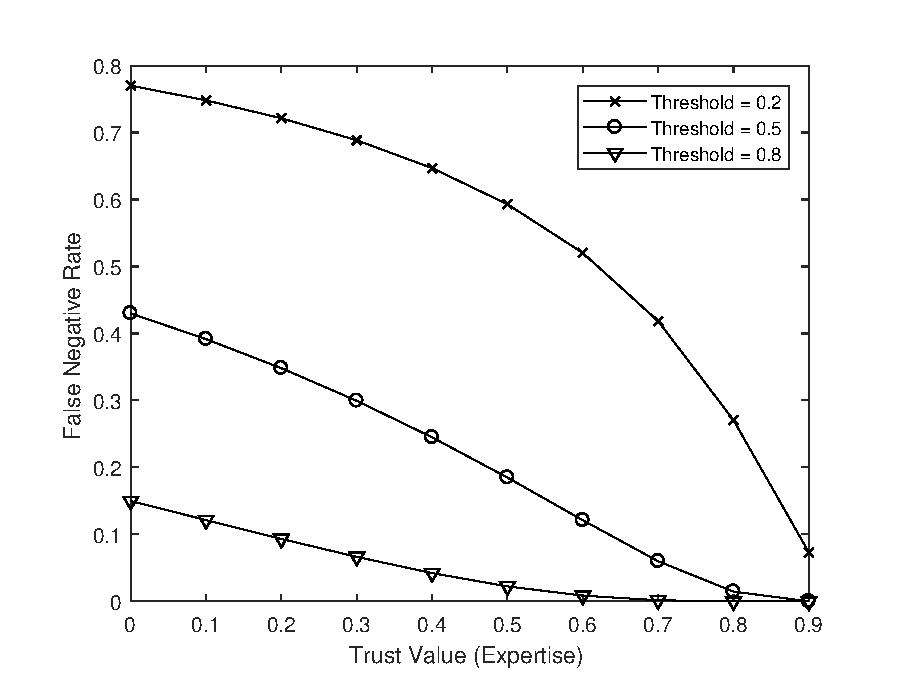
\includegraphics{fnt.eps}}
\caption{False Negative vs. Trust Value t .}
\label{fig4}
\end{figure}

\begin{figure}[htbp]

\centering
\scalebox{0.45}{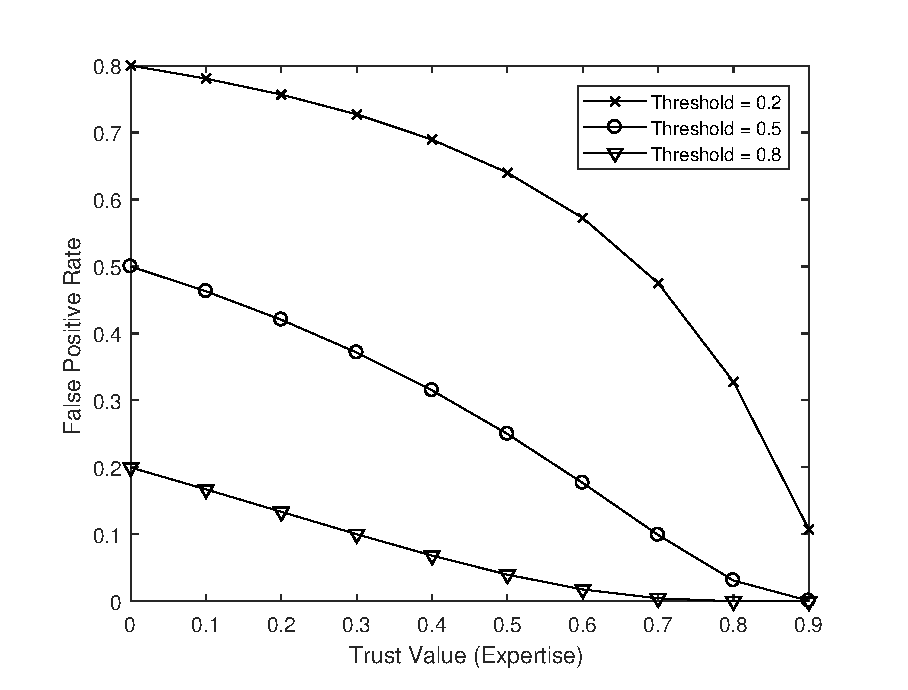
\includegraphics{fpt.eps}}
\caption{False Positive vs. Trust Value t.}
\label{fig5}
\end{figure}


\begin{figure}[htbp]

\centering
\scalebox{0.45}{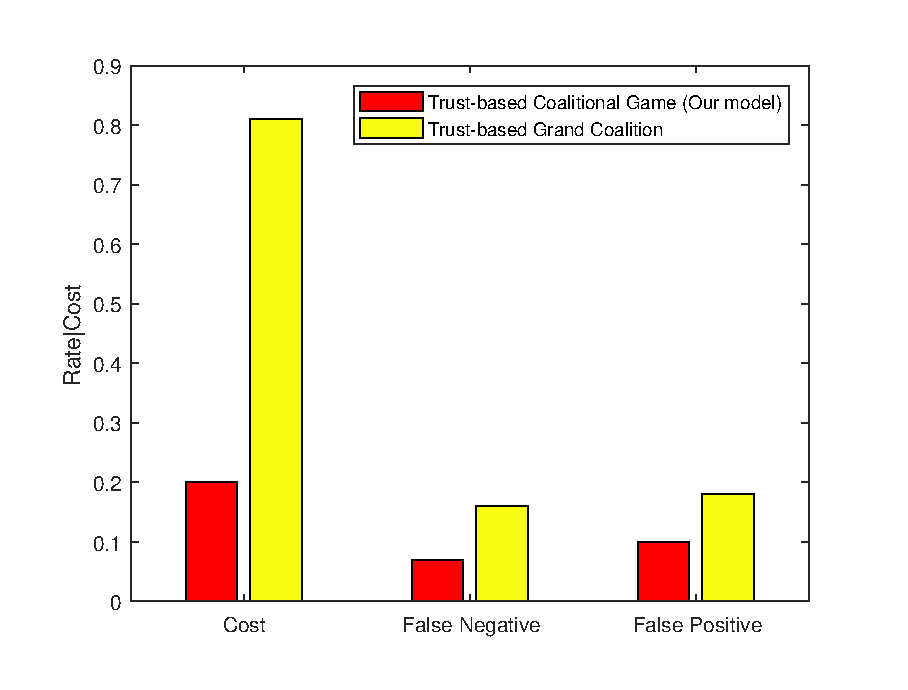
\includegraphics{cost.eps}}
\caption{Comparison of two coalition formation models.}
\label{fig6}
\end{figure}


Fig. \ref{fig6} gives a comparison between the proposed trust-based coalitional game approach and the trust-based grand coalition approach. The latter considers all existing IDSs during the cooperation. In other words, the coalition is done among all IDSs. Thus, the feedback is received from all IDSs and the final decisions are made using the same proposed aggregation model (i.e., Dempster-Shafer). This is unlike our approach where we first run a coalition formation Algorithm (Algorithm 1) and minimise the number of IDSs inside the coalition. The figure shows the superiority of the proposed model for both the false positive and false negative rates. This is due to the fact that the proposed coalition approach minimises the number of untrusted IDSs inside each generated coalition. Thus, the received feedback is more likely to reflect the real status of any suspicious behaviour, whether it is a real attack or not. However, for the grand coalition approach, the feedback is received from every existing IDS. Therefore, there will be a chance of receiving incorrect feedback from untrusted IDSs.  Fig. \ref{fig6} also studies the cost associated with using each approach. The cost represents the time needed to make a judgment about a suspicious attack. The result is projected in a range between 0 and 1. Our model yields a minimum overhead compared to the grand coalition approach. The reason is that our model minimises unnecessary consultation requests by consulting only those trusted IDSs in the final coalition. This is unlike the grand coalition approach where a consultation request is sent to all existing IDSs.



\section{Conclusion}

\label{sec:Conclusion}


This paper investigates a novel trust-based cooperative IDS in a multi-cloud environment. To this end, we propose a cooperative game-theoretic framework. The framework enables an IDS to evaluate the trust value of other IDSs using bayesian inference. We devise a coalition formation algorithm, that is based on the coalitional game theory. The algorithm enables IDSs to leave or join a given coalition in such a way that enhances their ability to work with trusted IDSs. The proposed algorithm converges to a Nash-stable situation; that is, no IDS has an incentive to leave its current coalition to move to another coalition. Furthermore, we propose a feedback aggregation algorithm, that is based on Dempster-Shafer Theory (DST), to enable an IDS inside a coalition to aggregate feedbacks about suspicious attacks in order to make the optimal decision in terms of detection accuracy. Numerical results show the effectiveness of the proposed approach in terms of false positive and false negative rates, and cost.

\section*{Acknowledgment}
The financial support of the Natural Sciences and Engineering
Research Council of Canada is gratefully acknowledged.


% trigger a \newpage just before the given reference
% number - used to balance the columns on the last page
% adjust value as needed - may need to be readjusted if
% the document is modified later
%\IEEEtriggeratref{8}
% The "triggered" command can be changed if desired:
%\IEEEtriggercmd{\enlargethispage{-5in}}

% references section

% can use a bibliography generated by BibTeX as a .bbl file
% BibTeX documentation can be easily obtained at:
% http://www.ctan.org/tex-archive/biblio/bibtex/contrib/doc/
% The IEEEtran BibTeX style support page is at:
% http://www.michaelshell.org/tex/ieeetran/bibtex/
%\bibliographystyle{IEEEtran}
% argument is your BibTeX string definitions and bibliography database(s)
%\bibliography{IEEEabrv,../bib/paper}
%
% <OR> manually copy in the resultant .bbl file
% set second argument of \begin to the number of references
% (used to reserve space for the reference number labels box)

%\begin{thebibliography}{1}
%
%\bibitem{IEEEhowto:kopka}
%H.~Kopka and P.~W. Daly, \emph{A Guide to \LaTeX}, 3rd~ed.\hskip 1em plus
%  0.5em minus 0.4em\relax Harlow, England: Addison-Wesley, 1999.
%
%\end{thebibliography}

\bibliographystyle{IEEEtran}
\bibliography{References}


% that's all folks
\end{document}


